\section{Grafsk bruger interface}
\textit{Dette afsnit omhandler design, implementering og test af GUI, til visualisering af de udførte aktiviteter. Først designes GUI til det specifikke formål udfra dets kravspecifikationer, hvorefter denne kan implementeres. Afslutningsvist bliver GUI testet i forhold til opstillede krav.}
\subsection{Design}
GUI benyttes til at motivere børn til en mere aktiv hverdag. Dette gøres ud fra \secref{motivation_boern}, hvor det beskrives at børn motiveres gennem succesoplevelser. GUI designes dermed ud fra at alle børn har mulighed for at optjene mange point, da pointene vægtes ud fra intensiteten, tiden samt typen af aktivitet.

Data fra algoritmerne vedrørende aktiviteterne gang, løb og cykling sendes til MATLAB, som det ses på \figref{fig:GUI}. Fra algoritmen vedrørende gang og løb sendes der to resultater. Resultaterne består i en peakværdi og et resultat af varighed siden sidst detekterede peak. Peakets værdi informere om hvilken aktivitet på baggrund af dets størrelse, varigheden bør tillægges. Fra algoritmen vedrørende cykling sendes der et resultat til MATLAB bestående af varigheden for udført cykling. Fra algoritmen vedrørende pulssensoren sendes data i form af BPM, beregnet over tre peaks. \\
Der er fastsat en tærskelværdi for gang, løb og cykling, hvoraf GUI modtager resultater fra algoritmerne. Ved gang, løb og cykling modtages varigheden som samples og skal dermed omregnes til tid. For at omregne dette til en faktor bestående af tid, skal det modtagne resultat divideres med samplingsfrekvensen. Herefter ligges tiden over i en tidsvariabel for den tilhørende aktivitet. Denne vises som værdi for den enkelte aktivitet, så det er muligt at se hvor længe barnet har været aktiv ved de forskellige aktiviteter.

Hver aktivitet belønnes forskelligt, da det er væsentligt at få børnene til at løbe og cykle mere, end blot at gå. Dermed ganges tiden for løb med tre, for cykling med to og for gang med en. Derudover belønnes barnet for intensiteten af aktiviteten. Aktivitetens point ganges med to ved høj intensitet, ganges med 1,5 ved moderat intensitet, og ganges ikke ved lav intensitet. Pointene visualiseres ud for den enkelte aktivitet, så barnet kan se hvor mange point de har opnået ved udførslen for den enkelte aktivitet igennem en hel dag. For at aktivere børnene hver dag, samles dagens point for alle aktiviteter udført i løbet af dagen. Pointene vises grafisk som en søjle hvormed barnet nemt kan få et overblik over antallet af point fra de forskellige dage. Søjlen afspejler hvor mange point børnene har opnået samt hvor stor en del der er opnået ved henholdsvis gang, løb og cykling.  

\begin{figure}[H]
	\centering
	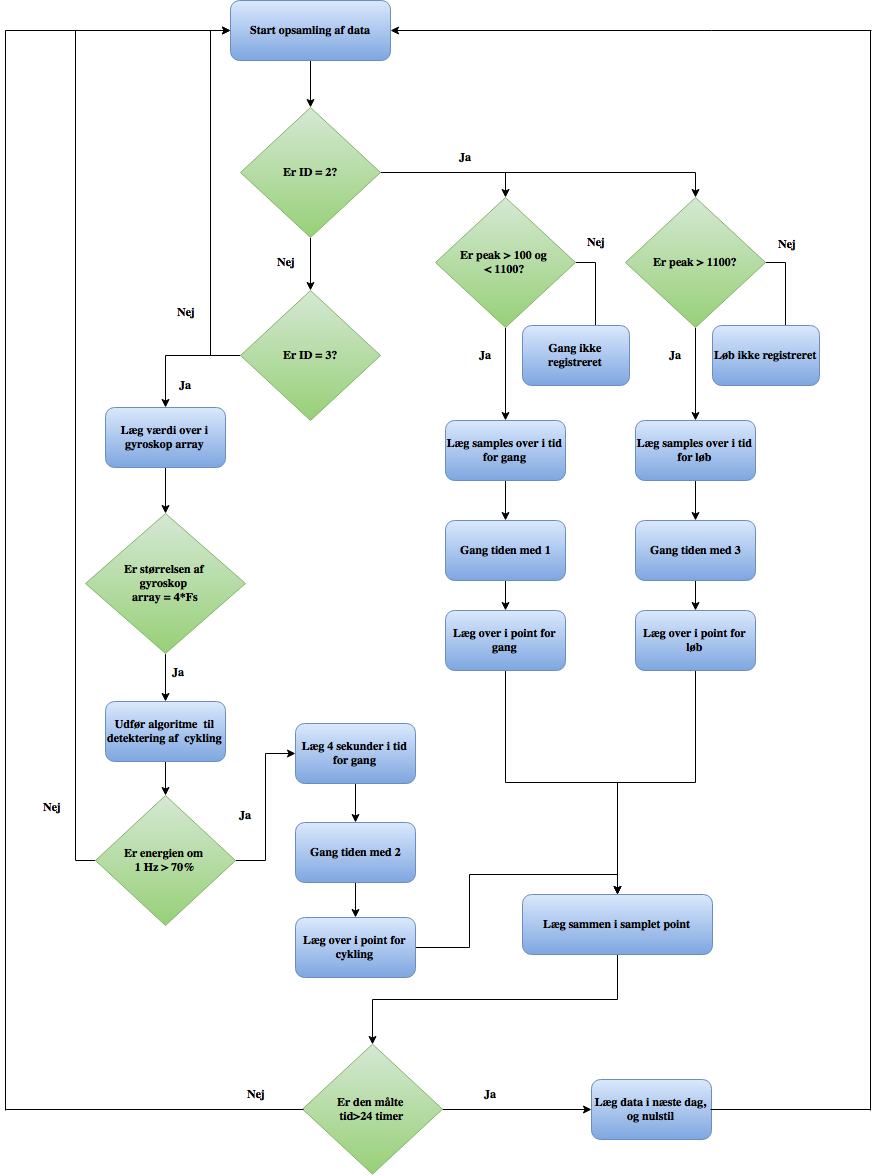
\includegraphics[scale=0.4]{figures/cDesign/pseudo_GUI.png}
	\caption{På figuren ses et flowchart som gennemgår hvorledes resultaterne fra de forskellige algoritmer behandles af GUI.}
	\label{fig:GUI}
\end{figure}

\subsection{Implementering}
GUI implementeres ved at anvende MATLABS funktion Graphical User Interface Design Environment (GUIDE) som er en funktion der gør det muligt at lave en specifik brugerflade. I GUIen benyttes en toggle button for at starte og slutte indsamling af resultater fra algoritmerne vedrørende aktiviteterne gang, løb og cykling. Derudover benyttes axes, som benyttes til at repræsentere de samlede point der er samlet i løbet af dagen. Sidst benyttes static text til de resterende funktioner i GUI. \newline
Resultaterne fra algoritmerne hentes ind til MATLAB, hvor de gemmes i en variabel med [samples,peak,BPM].

\subsubsection{Test}
GUIs funktionalitet tests ud fra kravene heraf, se \secref{krav_GUI}
Den trådløse kommunikation testes ud fra kravene hertil, se \secref{krav_BLE}. Der undersøges kvaliteten af forbindelsen mellem GAP peripheral og GAP central i forhold til afstand. GAP peripheral bliver sat til at videresende datapakker, som GAP central skal modtage alle af. Hvis dataoverførslen er nøjagtig, vil der ikke mangle nogle pakker. Dette vil blive illustreret igennem MATLAB, hvori en nøjagtig overførsel vil medføre en fuldstændig lineær kurve. Hvis datapakker er gået tabt, vil illustrationen af antal modtagne pakker varierer fra antal sendte pakker med stor hældning, og den kurven vil ikke være lineær. Denne test udføres med forskellig afstand mellem GAP peripheral og GAP central, hvoraf den maksimale afstand for succesfuld dataoverførsel vil komme til udtryk. \\
Datapakkerne i denne test sendes fire gange i sekundet, og resultaterne bliver opsamlet igennem 30 sekunder. Der skabes forbindelse mellem GAP peripheral og GAP central, hvor antallet af modtagne datapakker optages igennem RealTerm. Derfra konverteres det fra hex til decimaltal, hvormed data kan plottes i matlab.\fxnote{capture, optaget i hex, konverteret til decimaltal, som er plottet i matlab}